\subsection{ \og Stigmergie \fg{} }

Dans le but de bien dissocier la logique liée à la réflexion de celle qui structure le jeu, nous avons choisi de suivre le paradigme \og Agent et Environnement \fg{}. Notre IA est assimilée à un agent qui évolue dans un environnement qu'il peut observer et modifier.

Toute communication entre agents se fait donc par \og Tableau Noir \fg{}, c'est à dire en laissant des traces dans cet environnement partagé. Cette interaction dite \og Stigmergique\footnote{La stigmergie est une méthode de communication indirecte dans un environnement émergent auto-organisé, où les individus communiquent entre eux en modifiant leur environnement. (Article \og Stigmergie \fg{} de Wikipédia en français, licence CC-BY-SA)} \fg{} est nécessairement asynchrone mais possède l'avantage de ne nécessiter qu'un seul canal de communication par agent. Ce canal, qui relie l'agent à son environnement, est bidirectionnelle : il permet à l'agent de recevoir des stimuli et d'envoyer des impulsions. Dans la suite de ce document, nous parlerons de \og percepts\fg{} et \og actions\fg{}.

\begin{figure}[H] 
\centering
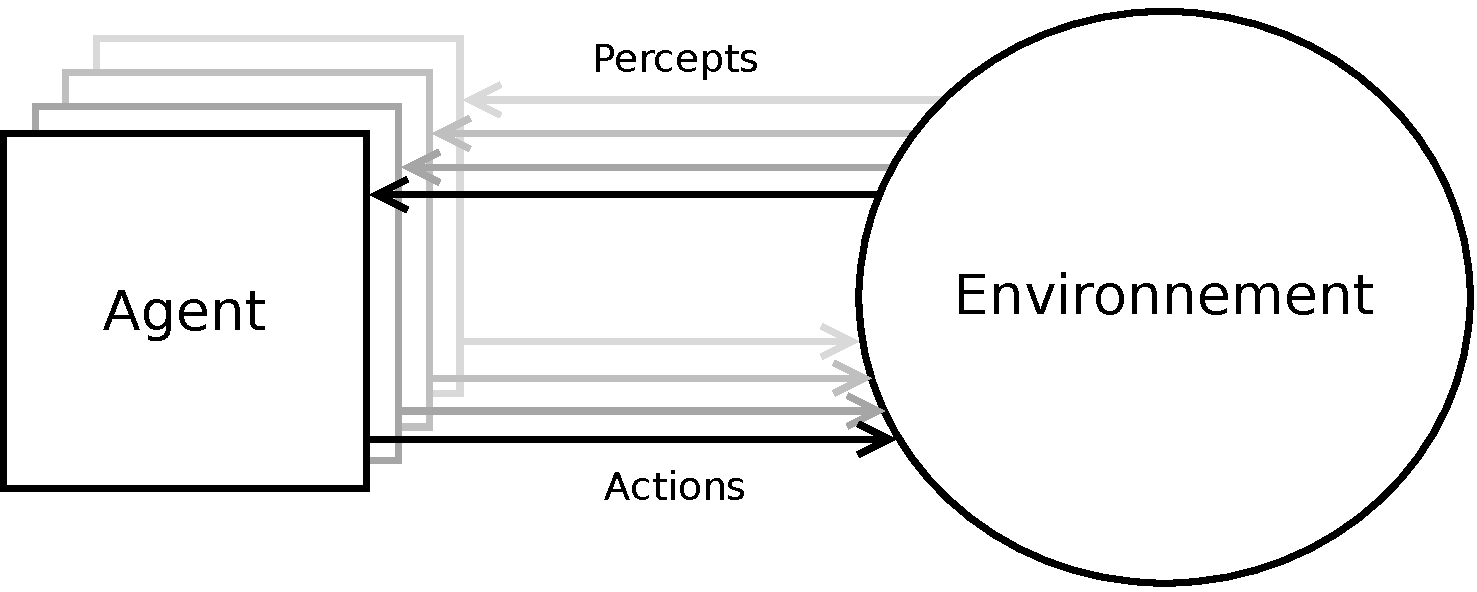
\includegraphics[width=\textwidth]{files/env/agent_env} 
\caption{Modèle \og Agent et Environnement \fg{}} 
\label{agent_env}
\end{figure}

La séparation entre l'agent et son environnement permet de gagner en flexibilité : la communication ne se faisant qu'au travers de l'envoie de messages précis, tout algorithme peut être encapsulé avec une interface simple pour en faire un agent.

L'agent peut donc être un humain ou une machine. Une machine pouvant exécuter notre modèle aussi bien qu'une intelligence artificielle tiers. 

Ainsi, nous disposons d'une abstraction du fonctionnement interne de chaque agent, ce qui permet
\begin{itemize}
\item d'une part de faire jouer notre agent contre un autre agent basé sur une stratégie connue, facilitant ainsi l'évaluation de notre modèle,
\item d'autre part de tester les développements qui concernent l'environnement avant même que notre IA ne soit fonctionnelle en faisant jouer des agents naïfs. Cette méthode permet d'isoler pleinement le développement de la plateforme de tests de celui de l'IA.
\end{itemize}

\subsection{ Agent \og Arbitre \fg{} }

Dans notre cas l'environnement est un jeu de plateau, donc une grille dont les cases peuvent contenir un pion ou être vide. L'environnement doit aussi "connaître", pour ainsi dire, quel est le prochain joueur qui doit jouer ainsi que toute autre information qui ne peut pas être directement déduite de l'état du plateau. Finalement il doit pouvoir juger de la légalité des coups proposés par l'agent, et par le même biais savoir comment initialiser le plateau de la bonne manière.
Il se décompose donc en trois modules: un plateau, une liste de règles et un processeur qui les manipule. Au lieu de briser le métaphore du \og Tableau Noir \fg{} en parlant d'environnement-agent, nous ce processeur sera en effet un agent tiers: une sorte d'arbitre neutre. C'est un agent purement réactif qui maintient l'état du jeu en exécutant les coups qui lui sont envoyés par les agents joueurs dans la mesure du légale. Il devrait bien-sur les notifier de l'éventuelle faillite de leurs actions, ainsi que leur envoyer l'état du plateau en cas de demande. 

\begin{figure}[H] 
\centering
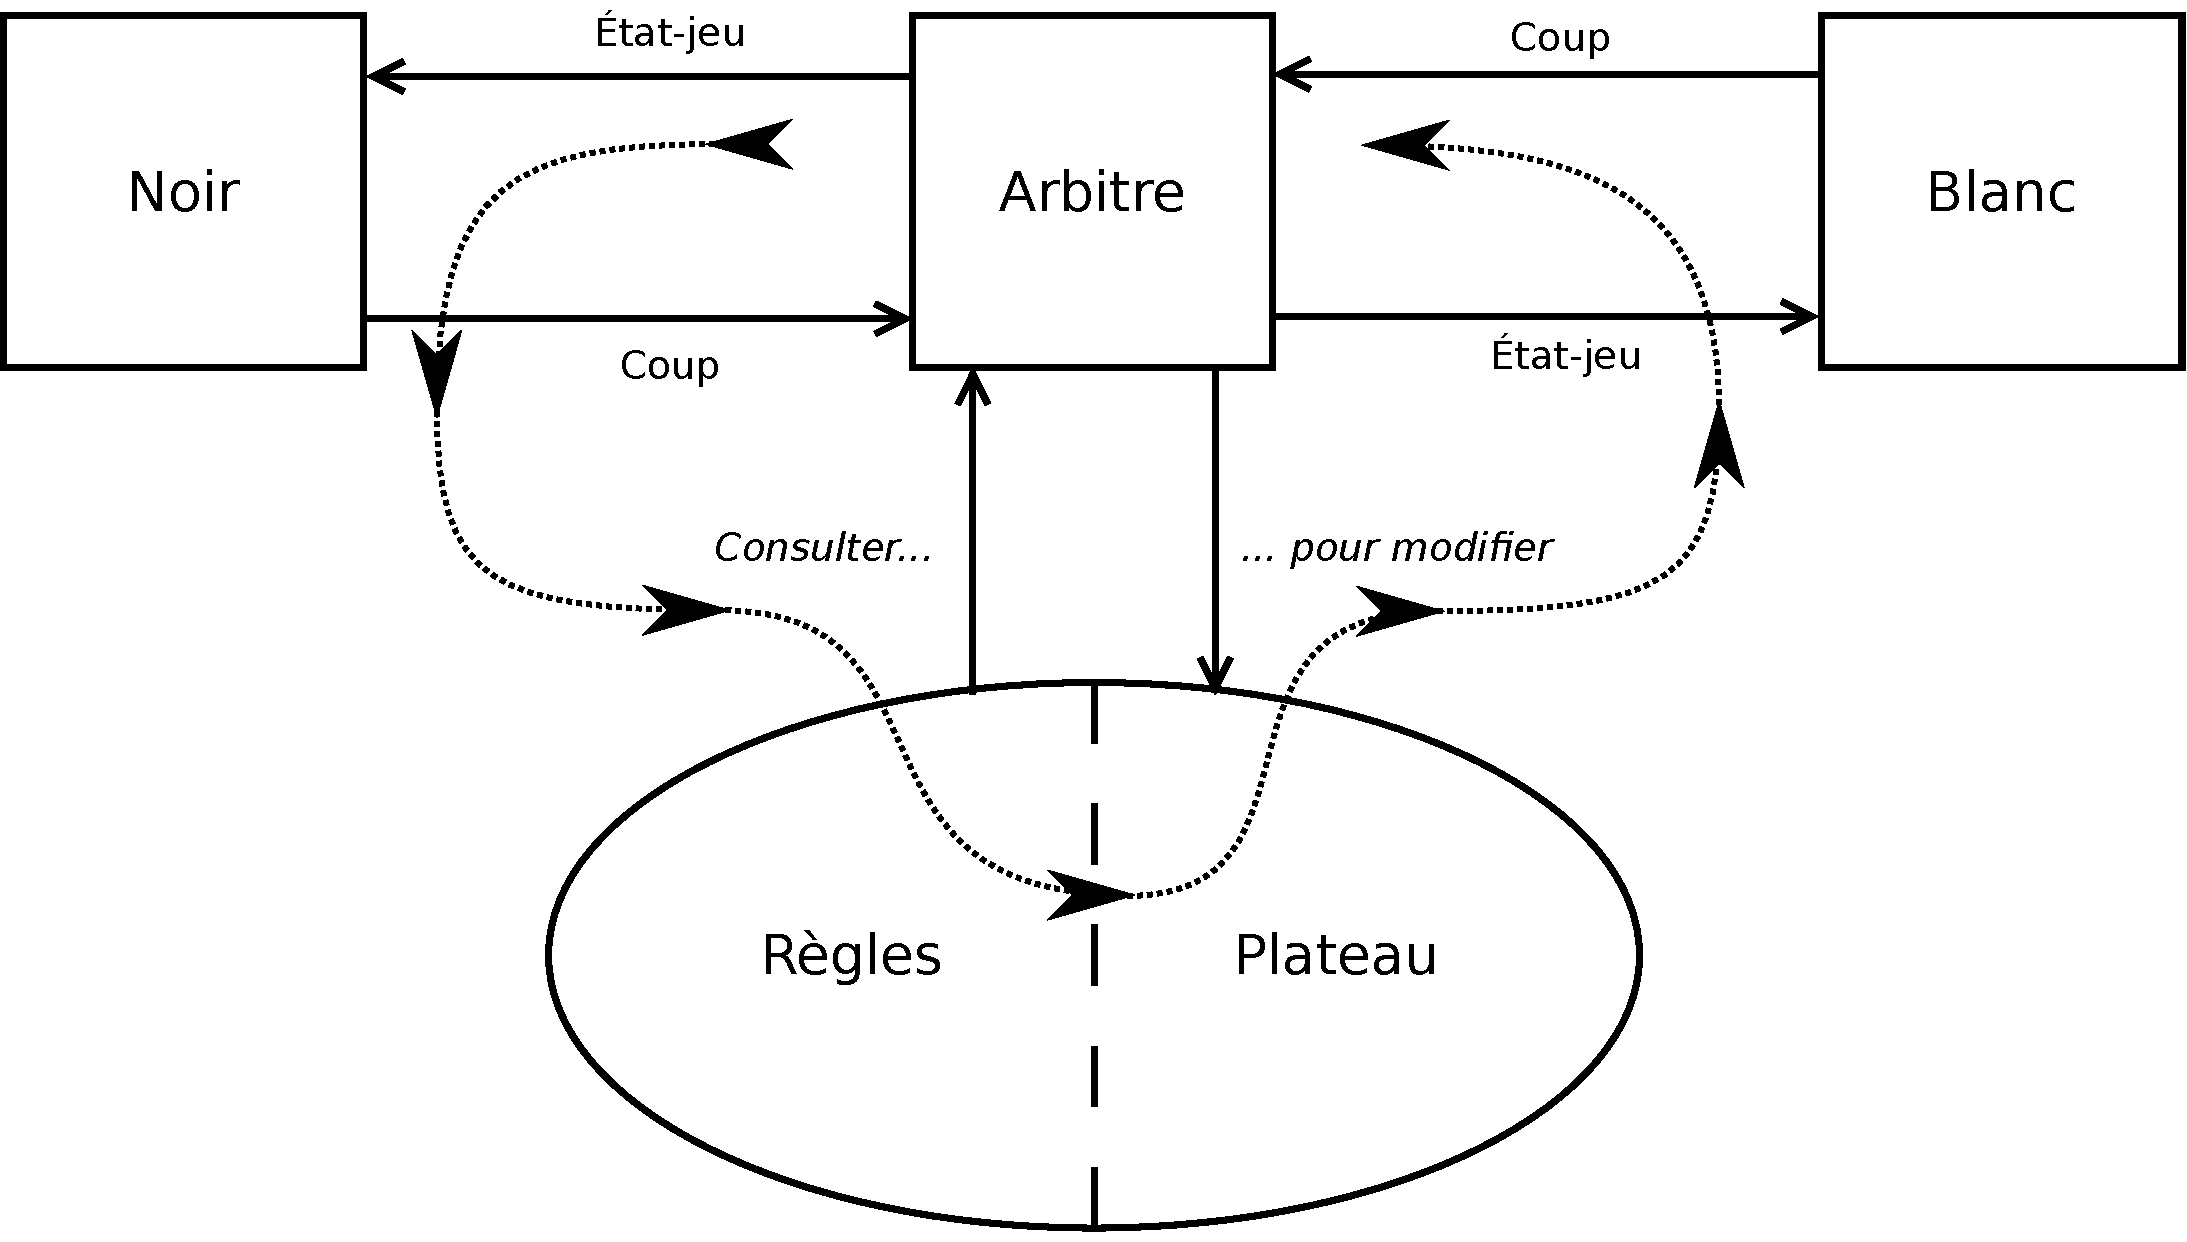
\includegraphics[width=\textwidth]{files/env/arbitre} 
\caption{Interactions entre l'Arbitre et les autres agents} 
\label{arbitre}
\end{figure}

Finalement c'est à travers cet agent-filtre que les autres iront modifier l'environnement et donc communiquer entre eux. Suite à cette étude préalable, il nous semble claire qu'une architecture client-serveur serait recommandé pour l'implémentation des interactions entre les agents et leur environnement.